%%%%%%%%%%%%%%%%%%%%%%%%%%%%%%%%%%%%%%%%%
% Beamer Presentation
% LaTeX Template
% Version 1.0 (10/11/12)
%
% This template has been downloaded from:
% http://www.LaTeXTemplates.com
%
% License:
% CC BY-NC-SA 3.0 (http://creativecommons.org/licenses/by-nc-sa/3.0/)
%
%%%%%%%%%%%%%%%%%%%%%%%%%%%%%%%%%%%%%%%%%

%----------------------------------------------------------------------------------------
%	PACKAGES AND THEMES
%----------------------------------------------------------------------------------------

\documentclass{beamer}

\mode<presentation> {

% The Beamer class comes with a number of default slide themes
% which change the colors and layouts of slides. Below this is a list
% of all the themes, uncomment each in turn to see what they look like.

%\usetheme{default}
%\usetheme{AnnArbor}
%\usetheme{Antibes}
%\usetheme{Bergen}
%\usetheme{Berkeley}
%\usetheme{Berlin}
%\usetheme{Boadilla}
%\usetheme{CambridgeUS}
%\usetheme{Copenhagen}
\usetheme{Darmstadt}
%\usetheme{Dresden}
%\usetheme{Frankfurt}
%\usetheme{Goettingen}
%\usetheme{Hannover}
%\usetheme{Ilmenau}
%\usetheme{JuanLesPins}
%\usetheme{Luebeck}
%\usetheme{Madrid}
%*\usetheme{Malmoe}
%\usetheme{Marburg}
%\usetheme{Montpellier}
%\usetheme{PaloAlto}
%\usetheme{Pittsburgh}
%\usetheme{Rochester}
%\usetheme{Singapore}
%\usetheme{Szeged}
%\usetheme{Warsaw}

% As well as themes, the Beamer class has a number of color themes
% for any slide theme. Uncomment each of these in turn to see how it
% changes the colors of your current slide theme.

%\usecolortheme{albatross}
%\usecolortheme{beaver}
%\usecolortheme{beetle}
%\usecolortheme{crane}
%\usecolortheme{dolphin}
%\usecolortheme{dove}
%\usecolortheme{fly}
%\usecolortheme{lily}
\usecolortheme{orchid}
%\usecolortheme{rose}
%\usecolortheme{seagull}
%\usecolortheme{seahorse}
%\usecolortheme{whale}
%\usecolortheme{wolverine}

%\setbeamertemplate{footline} % To remove the footer line in all slides uncomment this line
%\setbeamertemplate{footline}[page number] % To replace the footer line in all slides with a simple slide count uncomment this line

%\setbeamertemplate{navigation symbols}{} % To remove the navigation symbols from the bottom of all slides uncomment this line
}


\usepackage{graphicx} % Allows including images
\usepackage{booktabs} % Allows the use of \toprule, \midrule and \bottomrule in tables
\usepackage{xspace}
\usepackage{caption}
\usepackage{subfigure}
\usepackage[english,brazil]{babel}
\usepackage[utf8]{inputenc}

%Renomeia o nome padrao das figuras.
\renewcommand{\figurename}{Figura}
\renewcommand{\tablename}{Tabela}
%----------------------------------------------------------------------------------------
%	TITLE PAGE
%----------------------------------------------------------------------------------------

\title[Computação Gráfica]{Conversão Matricial Algoritmos de Anti-Aliasing} % The short title appears at the bottom of every slide, the full title is only on the title page

\author{Uéliton Freitas} % Your name
\institute[UFMS] % Your institution as it will appear on the bottom of every slide, may be shorthand to save space
{
Universidade Católica Dom Bosco - UCDB \\ % Your institution for the title page
\medskip
\textit{freitas.ueliton@gmail.com} % Your email address
}
\date{\today} % Date, can be changed to a custom date


\begin{document}

\begin{frame}
\titlepage % Print the title page as the first slide
\end{frame}

\begin{frame}
\frametitle{Sumário} % Table of contents slide, comment this block out to remove it
\tableofcontents % Throughout your presentation, if you choose to use \section{} and \subsection{} commands, these will automatically be printed on this slide as an overview of your presentation
\end{frame}




%----------------------------------------------------------------------------------------
%	PRESENTATION SLIDES
%----------------------------------------------------------------------------------------

%------------------------------------------------
\section{Introdução} 
%------------------------------------------------

%\section{Speeded-Up Robust Features - SURF} % A subsection can be created just before a set of slides with a common theme to further break down your presentation into chunks
%\section{Baf Of Features and Colors}

%\section{Refer\^encias}
%%%%%%%%%%%%%%%%%%%%%%%%%%%%%%%%%%%%%%%%%%%%%%%%%%%%%%%%%%%%%%%%%%%%%%%%%%%%%%%%%%%%%%%%%%
\begin{frame}
\frametitle{Introdução}

		\begin{figure}[!h]
			\begin{center}
			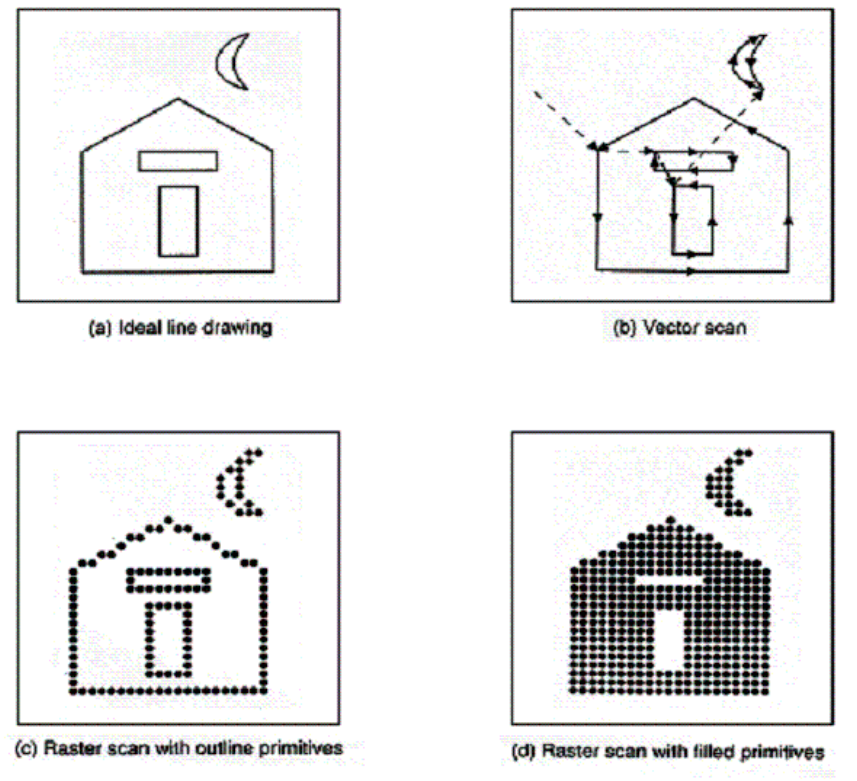
\includegraphics[width=0.6\textwidth]{Figures/IMG}
			\caption{Imagen vetorial $\times$ Imagem Matricial}
			\end{center}
		\end{figure}
	
\end{frame}



%%%%%%%%%%%%%%%%%%%%%%%%%%%%%%%%%%%%%%%%%%%%%%%%%%%%%%%%%%%%%%%%%%%%%%%%%%%%%%%%%%%%%%%%%%
\begin{frame}
\frametitle{Introdução}

		\begin{block}{Problemas}
		\begin{itemize}
			\item Traçar primitivas geométricas (segmentos de retas, polígonos, circunferências, elipses, curvas,...) no dispositivo matricial.
			\item ``rastering''= conversão vetorial $\to$ matricial.
			
			\item Como ajustar uma curva, definida como coordenadas reais em um sistema de coordenadas inteiras cujos ``pontos'' tem área associada. 						 
		\end{itemize}
	\end{block}
	
\end{frame}


%%%%%%%%%%%%%%%%%%%%%%%%%%%%%%%%%%%%%%%%%%%%%%%%%%%%%%%%%%%%%%%%%%%%%%%%%%%%%%%%%%%%%%%%%%
\begin{frame}
\frametitle{Introdução}

		\begin{block}{Problemas}
		\begin{itemize}
			\item Traçar primitivas geométricas (segmentos de retas, polígonos, circunferências, elipses, curvas,...) no dispositivo matricial.
			\item ``rastering''= conversão vetorial $\to$ matricial.
			
			\item Como ajustar uma curva, definida como coordenadas reais em um sistema de coordenadas inteiras cujos ``pontos'' tem área associada. 						 
		\end{itemize}
	\end{block}
	
\end{frame}

%%%%%%%%%%%%%%%%%%%%%%%%%%%%%%%%%%%%%%%%%%%%%%%%%%%%%%%%%%%%%%%%%%%%%%%%%%%%%%%%%%%%%%%%%%
\begin{frame}
\frametitle{Introdução}

		\begin{figure}[!h]
			\begin{center}
			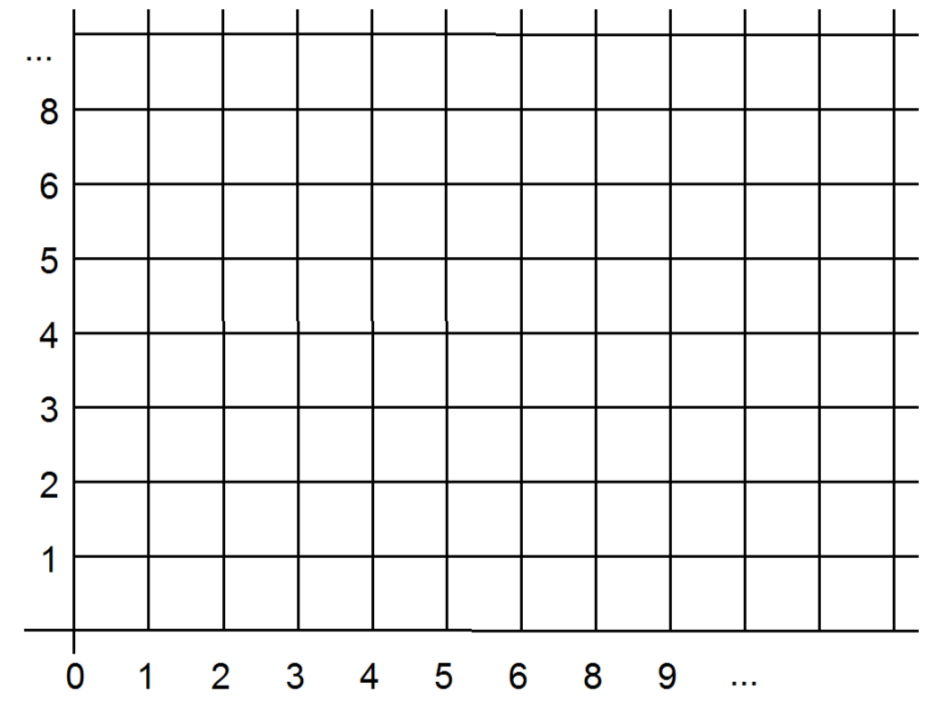
\includegraphics[width=0.6\textwidth]{Figures/DevSisCoo}
			\caption{Sistema de coordenadas de dispositivo.}
			\end{center}
		\end{figure}
	
\end{frame}


%%%%%%%%%%%%%%%%%%%%%%%%%%%%%%%%%%%%%%%%%%%%%%%%%%%%%%%%%%%%%%%%%%%%%%%%%%%%%%%%%%%%%%%%%%
\section{Conversão de Segmento de Reta}
\begin{frame}
\frametitle{Conversão de Segmento de Reta}

		\begin{block}{Conversão de Segmento de Reta}
		\begin{itemize}
			\item Dados pontos extremos em coordenadas de dispositivo
			\begin{itemize}
				\item $P_0 (x_0,y_0)$.
				\item $P_{end} (x_{end},y_{end})$.
			\end{itemize}
			\item Determinar quais pixels devem ser ``acesos'' para gerar uma boa aproximação do segmento de reta ideal.
		\end{itemize}
	\end{block}
	
\end{frame}

%%%%%%%%%%%%%%%%%%%%%%%%%%%%%%%%%%%%%%%%%%%%%%%%%%%%%%%%%%%%%%%%%%%%%%%%%%%%%%%%%%%%%%%%%%
\section{Conversão de Segmento de Reta}
\begin{frame}
\frametitle{Conversão de Segmento de Reta}

		\begin{block}{Conversão de Segmento de Reta}
		\begin{itemize}
			\item Características desejáveis:
			\begin{itemize}
				\item Linearidade.
				\item Precisão.
				\item Espessura (Densidade Uniforme).
				\item Intensidade independente de inclinação.
				\item Continuidade.
				\item Rapidez.
			\end{itemize}
		\end{itemize}
	\end{block}
	
\end{frame}

%%%%%%%%%%%%%%%%%%%%%%%%%%%%%%%%%%%%%%%%%%%%%%%%%%%%%%%%%%%%%%%%%%%%%%%%%%%%%%%%%%%%%%%%%%
\begin{frame}
\frametitle{Conversão de Segmento de Reta}

		\begin{block}{Equação da Reta}
		\begin{itemize}
			\item Usar equação explícita da reta
			\begin{equation*}
				y = m \cdot x + b
			\end{equation*}
			\item $m$ é a inclinação da reta e é dado por
			\begin{equation*}
				m = \frac{y_{end} - y_0}{x_{end} - x_0}
			\end{equation*}
			\item $b$ é a intersecção do eixo $y$ e dado por
			\begin{equation*}
				b = y_0 - m\cdot x_0
			\end{equation*}
		\end{itemize}
	\end{block}
	
\end{frame}

%%%%%%%%%%%%%%%%%%%%%%%%%%%%%%%%%%%%%%%%%%%%%%%%%%%%%%%%%%%%%%%%%%%%%%%%%%%%%%%%%%%%%%%%%%
\begin{frame}
\frametitle{Conversão de Segmento de Reta}

		\begin{block}{Algoritmos Simples}
		\begin{itemize}
			\item Varia-se $x$ unitariamente de pixel em pixel, encontrando o valor de $y$.
		\end{itemize}
	\end{block}
	
	\begin{figure}[!h]
			\begin{center}
			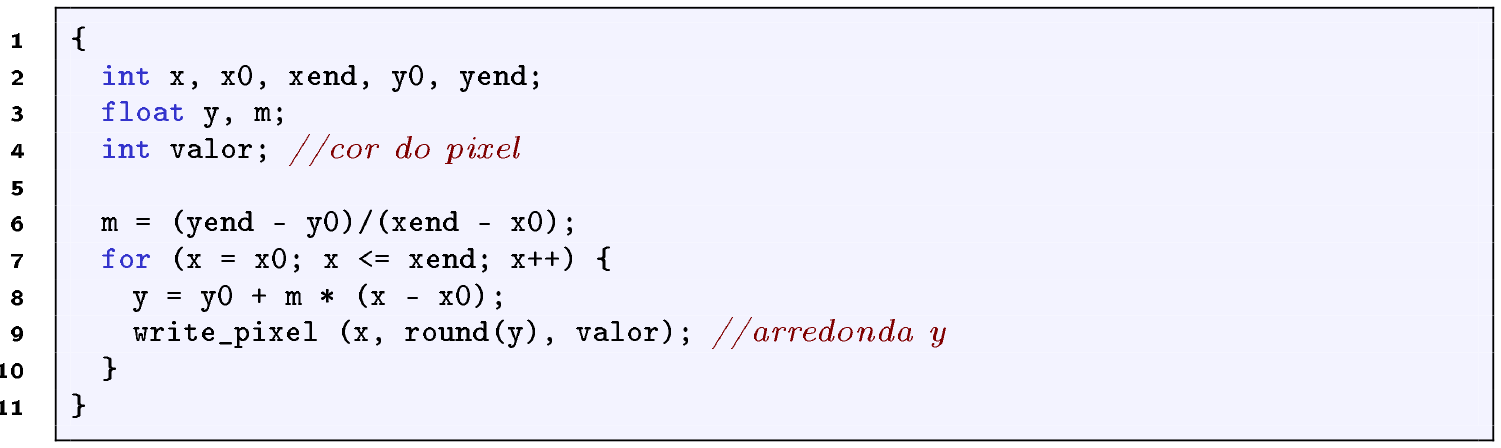
\includegraphics[width=1\textwidth]{Figures/Cod}
			\end{center}
		\end{figure}
	
\end{frame}


%%%%%%%%%%%%%%%%%%%%%%%%%%%%%%%%%%%%%%%%%%%%%%%%%%%%%%%%%%%%%%%%%%%%%%%%%%%%%%%%%%%%%%%%%%
\begin{frame}
\frametitle{Conversão de Segmento de Reta}

		\begin{block}{Algoritmos Simples}
		\begin{itemize}
			\item Na forma dada funciona apenas com segmentos em que $ 0 < m < 1$. Por que?
		\end{itemize}
	\end{block}
	
\end{frame}


%%%%%%%%%%%%%%%%%%%%%%%%%%%%%%%%%%%%%%%%%%%%%%%%%%%%%%%%%%%%%%%%%%%%%%%%%%%%%%%%%%%%%%%%%%
\begin{frame}
\frametitle{Conversão de Segmento de Reta}

		\begin{block}{Algoritmos Simples}
		\begin{itemize}
			\item Se $0 < m < 1$ a variação em $x$ é maior que em $y$. Caso não seja verdade, será traçado um segmento com buracos.
		\end{itemize}
	\end{block}
	
	\begin{figure}[!h]
			\begin{center}
			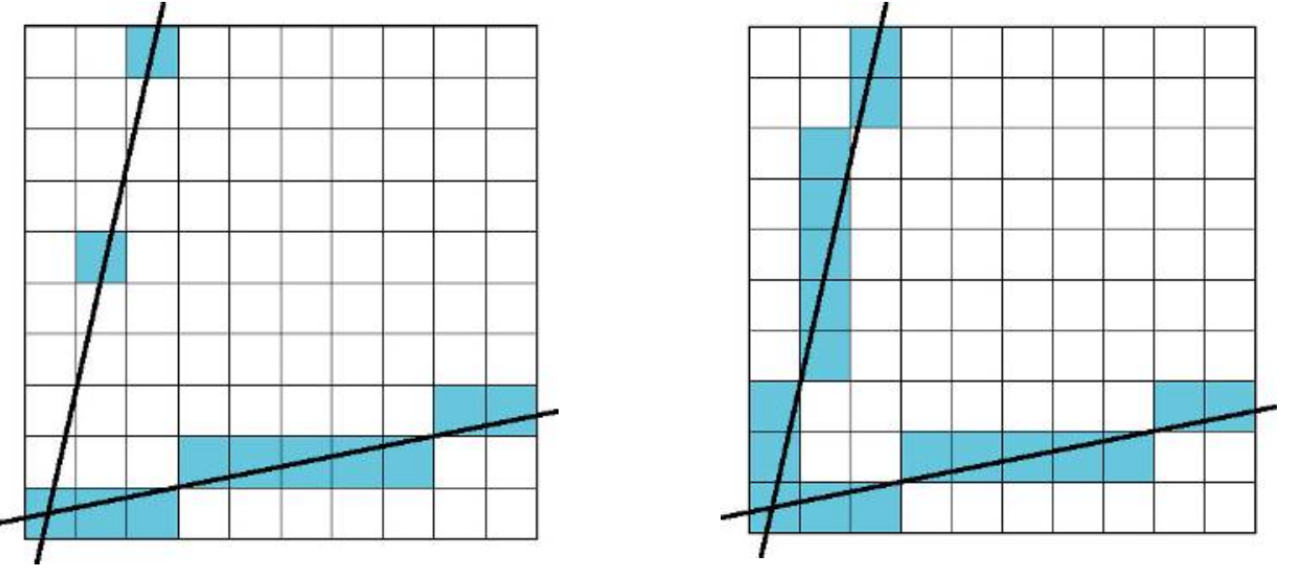
\includegraphics[width=1\textwidth]{Figures/Ret}
			\end{center}
		\end{figure}
	
\end{frame}

%%%%%%%%%%%%%%%%%%%%%%%%%%%%%%%%%%%%%%%%%%%%%%%%%%%%%%%%%%%%%%%%%%%%%%%%%%%%%%%%%%%%%%%%%%
\begin{frame}
\frametitle{Conversão de Segmento de Reta}

		\begin{block}{Algoritmos Simples}
		\begin{itemize}
			\item Se $m > 1$ basta inverter os papéis de $x$ e $y$, i.e, amostrar $y$ em intervalos unitários, e calcular $x$.
			\begin{equation*}
				x = x_0 + \frac{y-y_0}{m}
			\end{equation*}
		\end{itemize}
	\end{block}
	
\end{frame}


%%%%%%%%%%%%%%%%%%%%%%%%%%%%%%%%%%%%%%%%%%%%%%%%%%%%%%%%%%%%%%%%%%%%%%%%%%%%%%%%%%%%%%%%%%
\section{Digital Differential Analyzer (DDA) }
\begin{frame}
\frametitle{Digital Differential Analyzer (DDA)}

		\begin{block}{Digital Differential Analyzer (DDA)}
		\begin{itemize}
			\item Chamando $\delta x$ uma variação em $x$, podemos encontrar a variação $\delta y$ em $y$ correspondente fazendo:
			\begin{equation*}
				\delta y = m \cdot \delta x
			\end{equation*}
			\item ou similarmente
				\begin{equation*}
					\delta x = \frac{\delta y}{m}
				\end{equation*}
			\item O algoritmo DDA se baseia no cálculo de $\delta x$ e $\delta y$
		\end{itemize}
	\end{block}
	
\end{frame}

%%%%%%%%%%%%%%%%%%%%%%%%%%%%%%%%%%%%%%%%%%%%%%%%%%%%%%%%%%%%%%%%%%%%%%%%%%%%%%%%%%%%%%%%%%
\begin{frame}
\frametitle{Digital Differential Analyzer (DDA)}

		\begin{block}{Digital Differential Analyzer (DDA)}
		\begin{itemize}
			\item Para $|m| \leq 1$, na iteração $i$ temos:
				\begin{equation*}
					y_i = m \cdot x_i + b
				\end{equation*}
			\item Sendo $\delta_x$ a variação na direção de $x$, na iteração $i+1$ temos:
				\begin{align*}
					y_{i+1} &= m \cdot x_{i+1} + b \\
					y_{i+1} &= m \cdot (x_i + \delta_x) + b \\
					y_{i+1} &= m \cdot x_{i} + m \cdot \delta_x + b \\
					y_{i+1} &= (m \cdot x_{i} +b) + m \cdot \delta_x\\
					y_{i+1} &= y_i + m \cdot \delta_x
				\end{align*}
		\end{itemize}
	\end{block}
	
\end{frame}

%%%%%%%%%%%%%%%%%%%%%%%%%%%%%%%%%%%%%%%%%%%%%%%%%%%%%%%%%%%%%%%%%%%%%%%%%%%%%%%%%%%%%%%%%%
\begin{frame}
\frametitle{Digital Differential Analyzer (DDA)}

		\begin{block}{Digital Differential Analyzer (DDA)}
		\begin{itemize}
			\item Para $|m| \leq 1$, na iteração $i$ temos:
				\begin{equation*}
					y_{i+1} = y_i + m \cdot \delta_x
				\end{equation*}

			\item se $\delta_x = 1$ então:
				\begin{align*}
					x_{i+1} &= x_i + 1\\
					y_{i+1} &= y_i + m 
				\end{align*}
		\end{itemize}
	\end{block}
	
\end{frame}

%%%%%%%%%%%%%%%%%%%%%%%%%%%%%%%%%%%%%%%%%%%%%%%%%%%%%%%%%%%%%%%%%%%%%%%%%%%%%%%%%%%%%%%%%%
\begin{frame}
\frametitle{Digital Differential Analyzer (DDA)}

		\begin{block}{Digital Differential Analyzer (DDA)}
		\begin{itemize}
			\item Se $|m| > 1$, inverte-se os papéis, isto é, $\delta_y = 1$ e calcula-se $x$:
			\begin{align*}
				x_i 		&= \frac{y_i-b}{m} \\
				x_{i+1}	&= \frac{y_{i+1}-b}{m}\\
				x_{i+1}	&= \frac{y_i+\delta_y -b}{m}\\
				x_{i+1}	&= \frac{y_i-b}{m} + \frac{\delta_y}{m}\\
				x_{i+1}	&= x_i + \frac{\delta_y}{m}
			\end{align*}
		\end{itemize}
	\end{block}
\end{frame}

%%%%%%%%%%%%%%%%%%%%%%%%%%%%%%%%%%%%%%%%%%%%%%%%%%%%%%%%%%%%%%%%%%%%%%%%%%%%%%%%%%%%%%%%%%
\begin{frame}
\frametitle{Digital Differential Analyzer (DDA)}

		\begin{block}{Digital Differential Analyzer (DDA)}
		\begin{itemize}
			\item Se $|m| > 1$, inverte-se os papéis, isto é, $\delta_y = 1$ e calcula-se $x$:
			\begin{align*}
				x_{i+1}	&= x_i + \frac{\delta_y}{m}
			\end{align*}
			\item se $\delta_y=1$, então:
				\begin{align*}
					y_{i+1} &= y_i + 1 \\
					x_{i+1} &= x_i + \frac{1}{m}
				\end{align*}
		\end{itemize}
	\end{block}
\end{frame}

%%%%%%%%%%%%%%%%%%%%%%%%%%%%%%%%%%%%%%%%%%%%%%%%%%%%%%%%%%%%%%%%%%%%%%%%%%%%%%%%%%%%%%%%%%
\begin{frame}
\frametitle{Digital Differential Analyzer (DDA)}

		\begin{block}{Digital Differential Analyzer (DDA)}
		\begin{itemize}
			\item Assume-se que $x_0 < x_{end}$ e $y_0 < y_{end}$ ($m$ positivo), processando da esquerda para a direita.
			\item Se não é o caso, $\delta_x=-1$ ou $\delta_y=-1$, a equação deve ser adaptada.
			\begin{itemize}
				\item Fazer as adaptações como execícios.
			\end{itemize}
		\end{itemize}
	\end{block}
\end{frame}

%%%%%%%%%%%%%%%%%%%%%%%%%%%%%%%%%%%%%%%%%%%%%%%%%%%%%%%%%%%%%%%%%%%%%%%%%%%%%%%%%%%%%%%%%%
\begin{frame}
\frametitle{Digital Differential Analyzer (DDA)}

		\begin{block}{Exercício}
		\begin{itemize}
			\item Aplica o algoritmo de DDA para a conversão dos seguintes segmentos de retas:
				\begin{itemize}
					\item $P_1=(0,1),P_2=(5,3)$
					\item $P_1=(1,1),P_2=(3,5)$
				\end{itemize}
		\end{itemize}
	\end{block}
\end{frame}


%%%%%%%%%%%%%%%%%%%%%%%%%%%%%%%%%%%%%%%%%%%%%%%%%%%%%%%%%%%%%%%%%%%%%%%%%%%%%%%%%%%%%%%%%%
\section{Algoritmo de Bresenham}
\begin{frame}
\frametitle{Algoritmo de Bresenham}

		\begin{block}{Algoritmo de Bresenham}
		\begin{itemize}
			\item O algoritmo DDA apesar de ser incremental, envolve cálculos com números flutuantes (cálculo de $m$) sendo ineficiente.
			\item O algoritmo de Bresenham trabalha apenas com inteiros sendo mais eficiente.
		\end{itemize}
	\end{block}
\end{frame}

%%%%%%%%%%%%%%%%%%%%%%%%%%%%%%%%%%%%%%%%%%%%%%%%%%%%%%%%%%%%%%%%%%%%%%%%%%%%%%%%%%%%%%%%%%
\subsection{Retas}
\begin{frame}
\frametitle{Algoritmo de Bresenham}

		\begin{block}{Algoritmo de Bresenham (Retas)}
		\begin{itemize}
			\item Assume $ 0 < |m| < 1$.
			\item Incrementa $x$ em intervalos unitários, calcula o $y$ correspondente.
			\item Considera-se as duas possibilidades de escolha para $y$, decidindo qual a melhor.
			\begin{itemize}
				\item $(x_k,y_k) \to (x_{k+1},y_k)$
				\item $(x_k,y_k) \to (x_{k+1},y_{k+1})$
			\end{itemize}
		\end{itemize}
	\end{block}
\end{frame}


%%%%%%%%%%%%%%%%%%%%%%%%%%%%%%%%%%%%%%%%%%%%%%%%%%%%%%%%%%%%%%%%%%%%%%%%%%%%%%%%%%%%%%%%%%
\begin{frame}
\frametitle{Algoritmo de Bresenham}

		\begin{figure}[!h]
			\begin{center}
			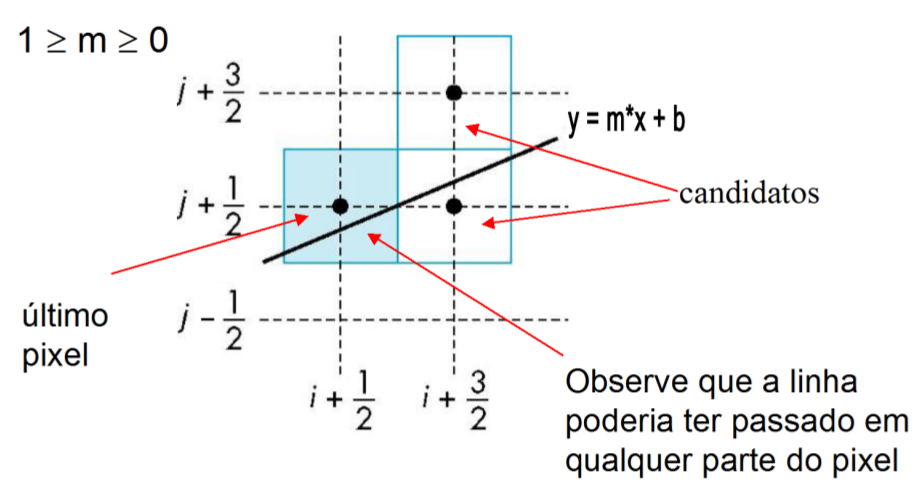
\includegraphics[width=1\textwidth]{Figures/Bre}
			\end{center}
		\end{figure}
\end{frame}

%%%%%%%%%%%%%%%%%%%%%%%%%%%%%%%%%%%%%%%%%%%%%%%%%%%%%%%%%%%%%%%%%%%%%%%%%%%%%%%%%%%%%%%%%%
\begin{frame}
\frametitle{Algoritmo de Bresenham}

		\begin{figure}[!h]
			\begin{center}
			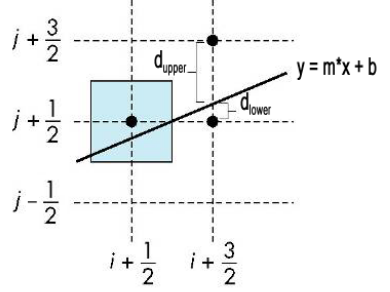
\includegraphics[width=0.5\textwidth]{Figures/Bre1}
			\end{center}
		\end{figure}
		\begin{block}{Algoritmo de Bresenham (Retas)}
		\begin{itemize}
			\item$ (d_{lower} - d_{upper} \geq 0) \to$ pixel superior.
			\item$ (d_{lower} - d_{upper} < 0) \to$ pixel inferior.
		\end{itemize}
	\end{block}
\end{frame}

%%%%%%%%%%%%%%%%%%%%%%%%%%%%%%%%%%%%%%%%%%%%%%%%%%%%%%%%%%%%%%%%%%%%%%%%%%%%%%%%%%%%%%%%%%
\begin{frame}
\frametitle{Algoritmo de Bresenham}
		\begin{block}{Algoritmo de Bresenham (Retas)}
		\begin{itemize}
			\item Com base na equação da reta ($y = m \cdot x + b$), na posição $x_k+1$, a coordenada $y$ é calculada da seguinte forma:
			\begin{equation*}
				y = m \cdot (x_k+1) + b
			\end{equation*}
			\item Então:
				\begin{align*}
					d_{lower} &= y - y_k \\
					d_{lower} &= m\cdot (x_k+1) +b -y_k
				\end{align*}
			\item e:
				\begin{align*}
					d_{upper} &= (y_k+1)-y \\
					d_{upper} &= y_k+1 - m \cdot (x_k+1) - b
				\end{align*}
		\end{itemize}
	\end{block}
\end{frame}

%%%%%%%%%%%%%%%%%%%%%%%%%%%%%%%%%%%%%%%%%%%%%%%%%%%%%%%%%%%%%%%%%%%%%%%%%%%%%%%%%%%%%%%%%%
\begin{frame}
\frametitle{Algoritmo de Bresenham}
		\begin{block}{Algoritmo de Bresenham (Retas)}
		\begin{itemize}
			\item Um teste rápido pode ser feito da seguinte forma para saber a proximidade:
					\begin{align}
						p_k &= d_{lower} - d_{upper} \\
						p_k &= 2m(x_k+1) - 2y_k+2b+1
					\end{align}
			\item Assim:
				\begin{itemize}
					\item $p_k > 0 \to$ pixel superior.
					\item $p_k < 0 \to$ pixel inferior. 
				\end{itemize}
		\end{itemize}
	\end{block}
\end{frame}


%%%%%%%%%%%%%%%%%%%%%%%%%%%%%%%%%%%%%%%%%%%%%%%%%%%%%%%%%%%%%%%%%%%%%%%%%%%%%%%%%%%%%%%%%%
\begin{frame}
\frametitle{Algoritmo de Bresenham}
		\begin{block}{Algoritmo de Bresenham (Retas)}
		\begin{itemize}
			\item Mas calcular $m$ é uma operação que ainda envolve ponto flutuante:
			\begin{equation*}
				m = \frac{y_{end} - y_0}{x_{end} - x_0} = \frac{\Delta_y}{\Delta_x}
			\end{equation*}
			\item Substituindo  $m$ por $\frac{\Delta_y}{\Delta_x}$, e multiplicando tudo por $\Delta_x$ em (1) temos:
			\begin{equation*}
				p_k = \Delta x (d_{lower} - d_{upper} )
			\end{equation*}
			\item Como $\Delta x > 0$, o sinal de $p_k$ não é alterado, assim:
				\begin{equation*}
					p_k = 2 \Delta y \cdot x_k - 2 \Delta x \cdot y_k + c
				\end{equation*}
			\item com $c = 2\Delta y + \Delta x(2b-1)$ que é um parâmetro constante e independente da posição do pixel.
		\end{itemize}
	\end{block}
\end{frame}

%%%%%%%%%%%%%%%%%%%%%%%%%%%%%%%%%%%%%%%%%%%%%%%%%%%%%%%%%%%%%%%%%%%%%%%%%%%%%%%%%%%%%%%%%%
\begin{frame}
\frametitle{Algoritmo de Bresenham}
		\begin{block}{Algoritmo de Bresenham (Retas)}
		\begin{itemize}
			\item No passo $k+1$ temos:
			\begin{equation*}
				p_{k+1} = 2 \Delta y \cdot x_{k+1} - 2 \Delta x \cdot y_{k+1} + c
			\end{equation*}
			\item subtraindo $p_k$ em ambos os lados temos:
			\begin{align*}
				p_{k+1} - p_k &= (2 \Delta y \cdot x_{k+1} - 2 \Delta x \cdot y_{k+1} + c) - p_k \\
				p_{k+1} - p_k &= 2 \Delta y \cdot (x_{k+1} - x_k) - 2 \Delta x \cdot (y_{k+1} - y_k)
			\end{align*}
			\item e como $x_{k+1} = x_k+1$ (incremento unitário em $x$), então:
				\begin{equation*}
					p_{k+1} = p_k + 2 \Delta y - 2 \Delta x \cdot (y_{k+1} - y_k)
				\end{equation*}
		\end{itemize}
	\end{block}
\end{frame}

%%%%%%%%%%%%%%%%%%%%%%%%%%%%%%%%%%%%%%%%%%%%%%%%%%%%%%%%%%%%%%%%%%%%%%%%%%%%%%%%%%%%%%%%%%
\begin{frame}
\frametitle{Algoritmo de Bresenham}
		\begin{block}{Algoritmo de Bresenham (Retas)}
		\begin{itemize}
			\item Nesta equação:
				\begin{equation*}
					p_{k+1} = p_k + 2 \Delta y - 2 \Delta x \cdot (y_{k+1} - y_k)
				\end{equation*}
			\item $y_k+1-y_k$ será 0 ou 1 dependendo do sinal de $p_k$
			\item Se $p_k < 0$, então o próximo ponto ($x_k+1,y_k$) então:
			\begin{align*}
				& y_{k+1}-y_k = 0\\
				& p_k+1 = p_k + 2 \Delta y
			\end{align*}
			\item caso contrário o ponto será ($x_k+1,y_k+1$), assim:
			\begin{align*}
				& y_{k+1}-y_k = 1\\
				& p_k+1 = p_k + 2 \Delta y - 2 \Delta x
			\end{align*}
		\end{itemize}
	\end{block}
\end{frame}

%%%%%%%%%%%%%%%%%%%%%%%%%%%%%%%%%%%%%%%%%%%%%%%%%%%%%%%%%%%%%%%%%%%%%%%%%%%%%%%%%%%%%%%%%%
\begin{frame}
\frametitle{Algoritmo de Bresenham}
		\begin{block}{Algoritmo de Bresenham (Retas)}
		\begin{itemize}
			\item Este cálculo iterativo é realizado para cada posição de $x$ começando da esquerda para a direita.
			\item O ponto de partida é calculado como sendo
				\begin{equation*}
					p_0 = 2 \Delta y - \Delta x
				\end{equation*}
		\end{itemize}
	\end{block}
\end{frame}

%%%%%%%%%%%%%%%%%%%%%%%%%%%%%%%%%%%%%%%%%%%%%%%%%%%%%%%%%%%%%%%%%%%%%%%%%%%%%%%%%%%%%%%%%%
\begin{frame}
\frametitle{Algoritmo de Bresenham}

		\begin{figure}[!h]
			\begin{center}
			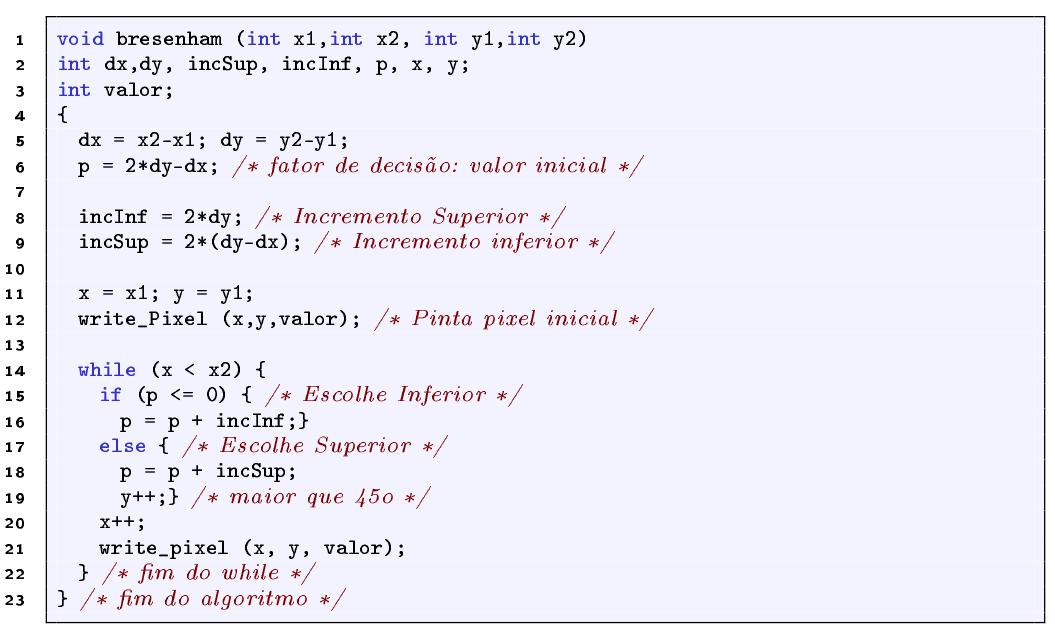
\includegraphics[width=1\textwidth]{Figures/AlgBre}
			\end{center}
		\end{figure}
\end{frame}

%%%%%%%%%%%%%%%%%%%%%%%%%%%%%%%%%%%%%%%%%%%%%%%%%%%%%%%%%%%%%%%%%%%%%%%%%%%%%%%%%%%%%%%%%%
\begin{frame}
\frametitle{Algoritmo de Bresenham}
		\begin{block}{Exercício}
		\begin{itemize}
			\item Aplique o algoritmo para a reta composta pelos seguintes pontos em seu extremo:
				\begin{itemize}
					\item $P_0(0,0)$
					\item $P_1(4,3)$
				\end{itemize}
		\end{itemize}
	\end{block}
\end{frame}

%----------------------------------------------------------------------------------------
\end{document} 